\begin{figure*}[t]
\centering
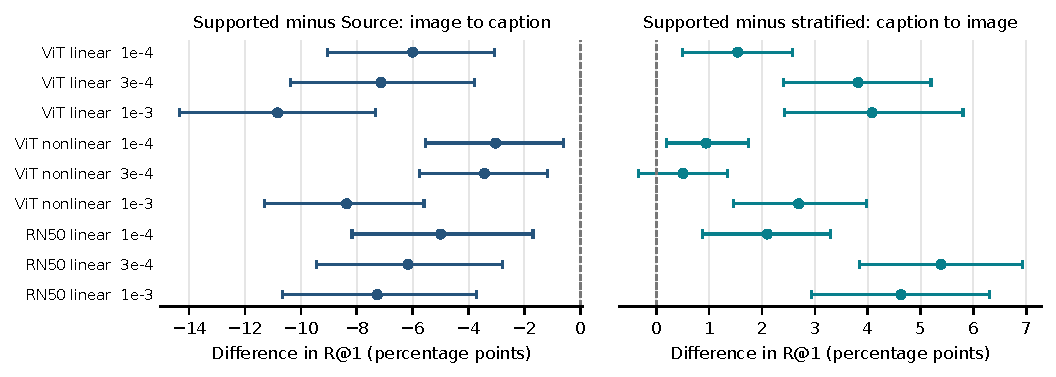
\includegraphics[width=\textwidth]{replication_summary_v5.pdf}
\caption{Caption identity and source retrieval at matched epoch ten. Dots average training seeds and fixed assignment draws. Bars show the adjusted intervals from each setting's separately declared comparison family. The appendix reports all retrieval directions and comparators.}\label{fig:newreplication}
\end{figure*}

\paragraph{The source-retrieval cost recurs across settings.}
Supported training reduces image-to-caption R@1 against Source at all three rates in both new replications.
The nonlinear effects are $-3.03$, $-3.43$, $-8.37$ percentage points across increasing rates.
The RN50 effects are $-5.00$, $-6.17$, $-7.27$ points.
Every adjusted interval lies below zero.
Figure~\ref{fig:newreplication} includes the original linear study and both new replications.
\paragraph{Caption identity helps the reverse direction.}
Against stratified promotion, RN50 gains $+2.10$, $+5.39$, $+4.63$ caption-to-image points.
All three adjusted lower bounds exceed zero.
The nonlinear gains are $+0.94$, $+0.51$, $+2.69$ points.
Its smallest and largest rates have positive lower bounds; the middle interval includes zero.
All RN50 image-to-caption intervals against stratified promotion include zero.
Nonlinear image-to-caption costs against stratified promotion have negative adjusted intervals at the two smaller rates.
Assignment benefits therefore depend on retrieval direction.
Appendix Tables~\ref{tab:nonlinearpartial} and~\ref{tab:rn50partial} report every new replication effect.
